% =========================================================
\section{Módulos das Unidades da Assessoria Legislativa}
\begin{frame}
	\frametitle{Módulos das Unidades}
	
	\begin{alertblock}{Módulos das Unidades}
		\begin{itemize}
			\item \textbf{Módulo ``Gerenciar Solicitações da Unidade''}: Acessível por ambos perfis; 
			\item \textbf{Módulo ``Área de Trabalho do Consultor Legislativo''}: Cada Consultor acessa a sua própria área de trabalho;
			\item \textbf{Módulo ``Minhas Notificações''}: Cada usuário do sistema pode acessar sua própria tela de notificações;
		\end{itemize}
	\end{alertblock}	
\end{frame}
% =========================================================
\section{Módulo Gerenciar Solicitações das Unidades}

\begin{frame}
	\frametitle{Módulos das Unidades}
	\framesubtitle{Módulo Gerenciar Solicitações das Unidades}
	\begin{figure}
		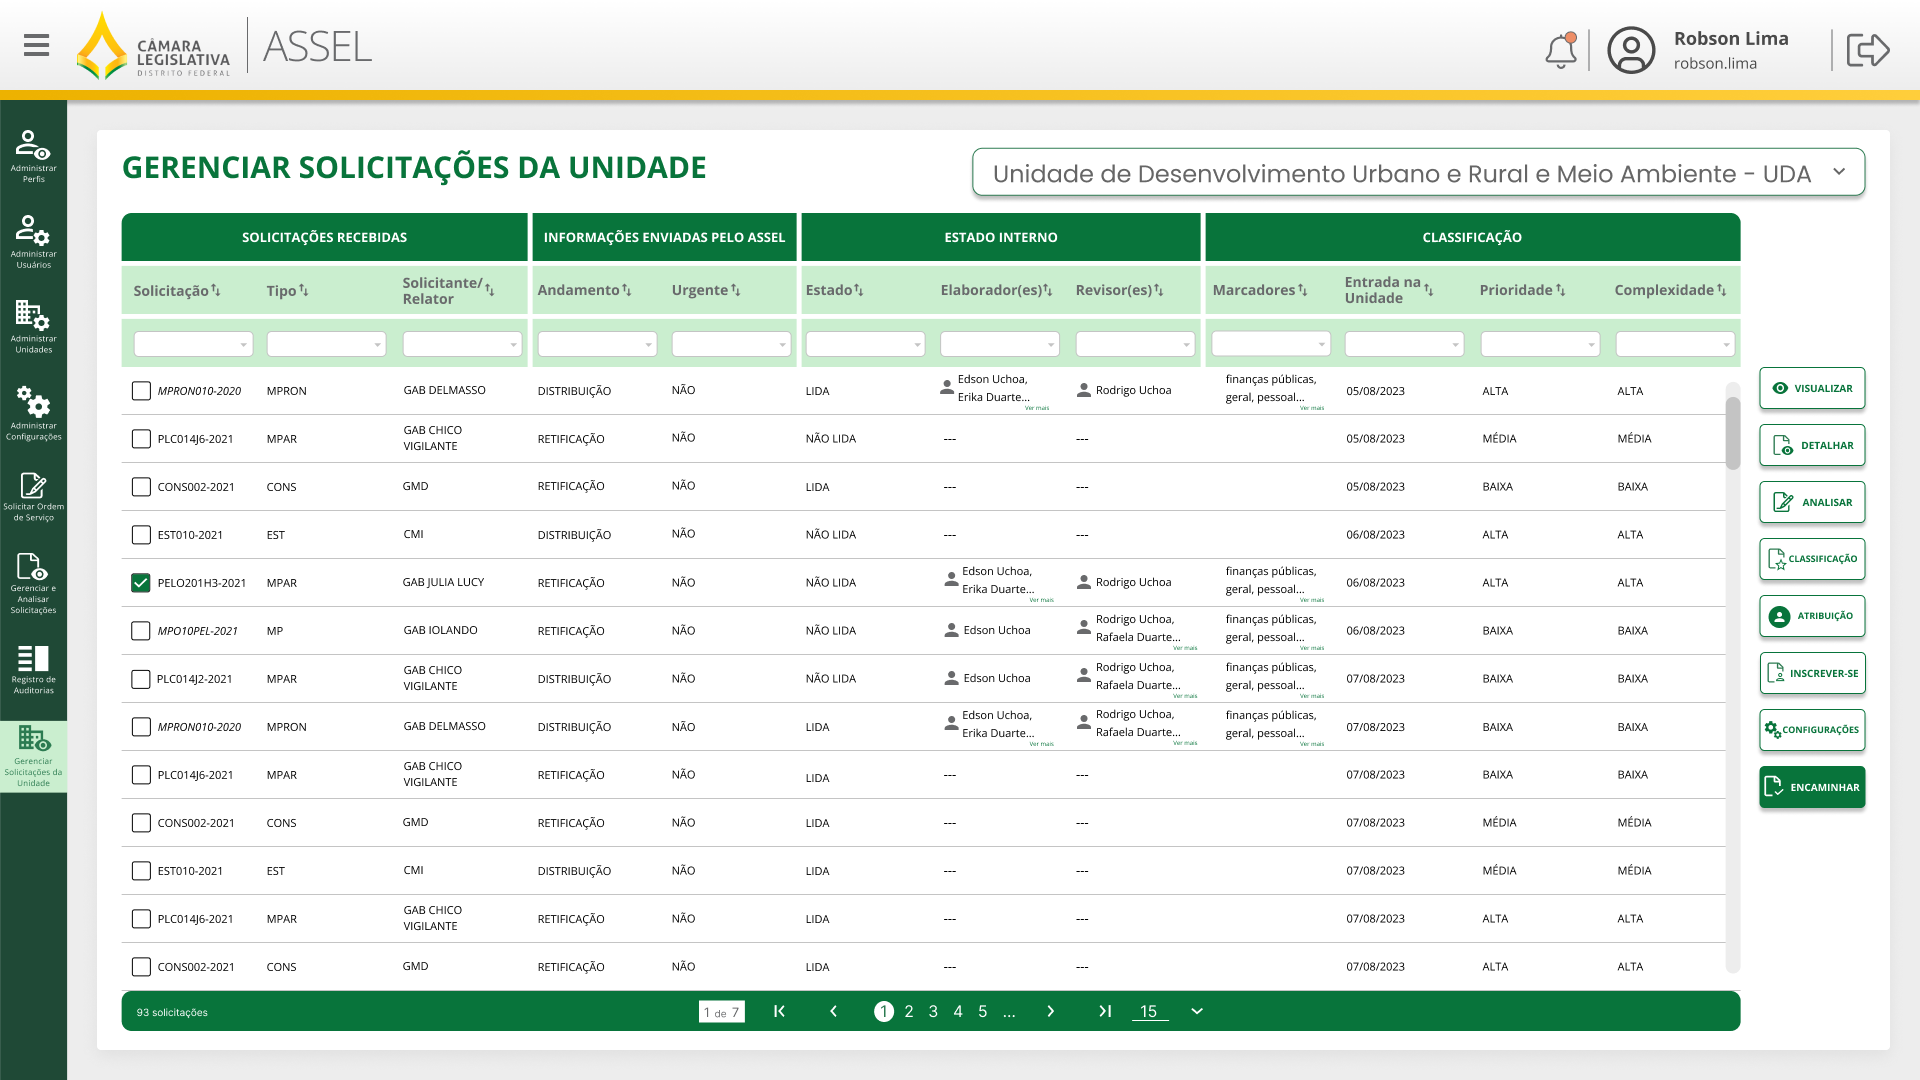
\includegraphics[width=0.99\linewidth]{GerSolUnid.png}
	\end{figure}
\end{frame}
% ------------------------------------------------------------
\begin{frame}
	\frametitle{Módulos das Unidades}
	\framesubtitle{Módulo Gerenciar Solicitações das Unidades - Objetivo}
	
	\begin{exampleblock}{Objetivo do ``Módulo Gerenciar Solicitações das Unidades''} 
		\begin{itemize}
			\item Gerenciamento pelos participantes da Unidade das solicitações que estão na carga de trabalho da Unidade.
		\end{itemize}
	\end{exampleblock}
\end{frame}
% ------------------------------------------------------------------
\begin{frame}
	\frametitle{Módulos das Unidades}
	\framesubtitle{Módulo Gerenciar Solicitações das Unidades}
	
	\begin{block}{Apresentação do Protótipo} % Block without title
		\begin{enumerate}
			\item Apresentar protótipo interativo do módulo;
			\item Explicar que cada Unidade da Assessoria Legislativa verá um módulo próprio e independente dos demais;
			\item Perfis:
			\begin{itemize}
				\item Supervisor
				\item Consultor Legislativo
			\end{itemize}
			
			\item Funcionalidades serão acessíveis de acordo com o perfil do usuário;
		\end{enumerate}
	\end{block}
\end{frame}
% =========================================================
\section{Módulo Área de Trabalho do Consultor Legislativo}

\begin{frame}
	\frametitle{Módulos das Unidades}
	\framesubtitle{Módulo Área de Trabalho do Consultor Legislativo}
	\begin{figure}
		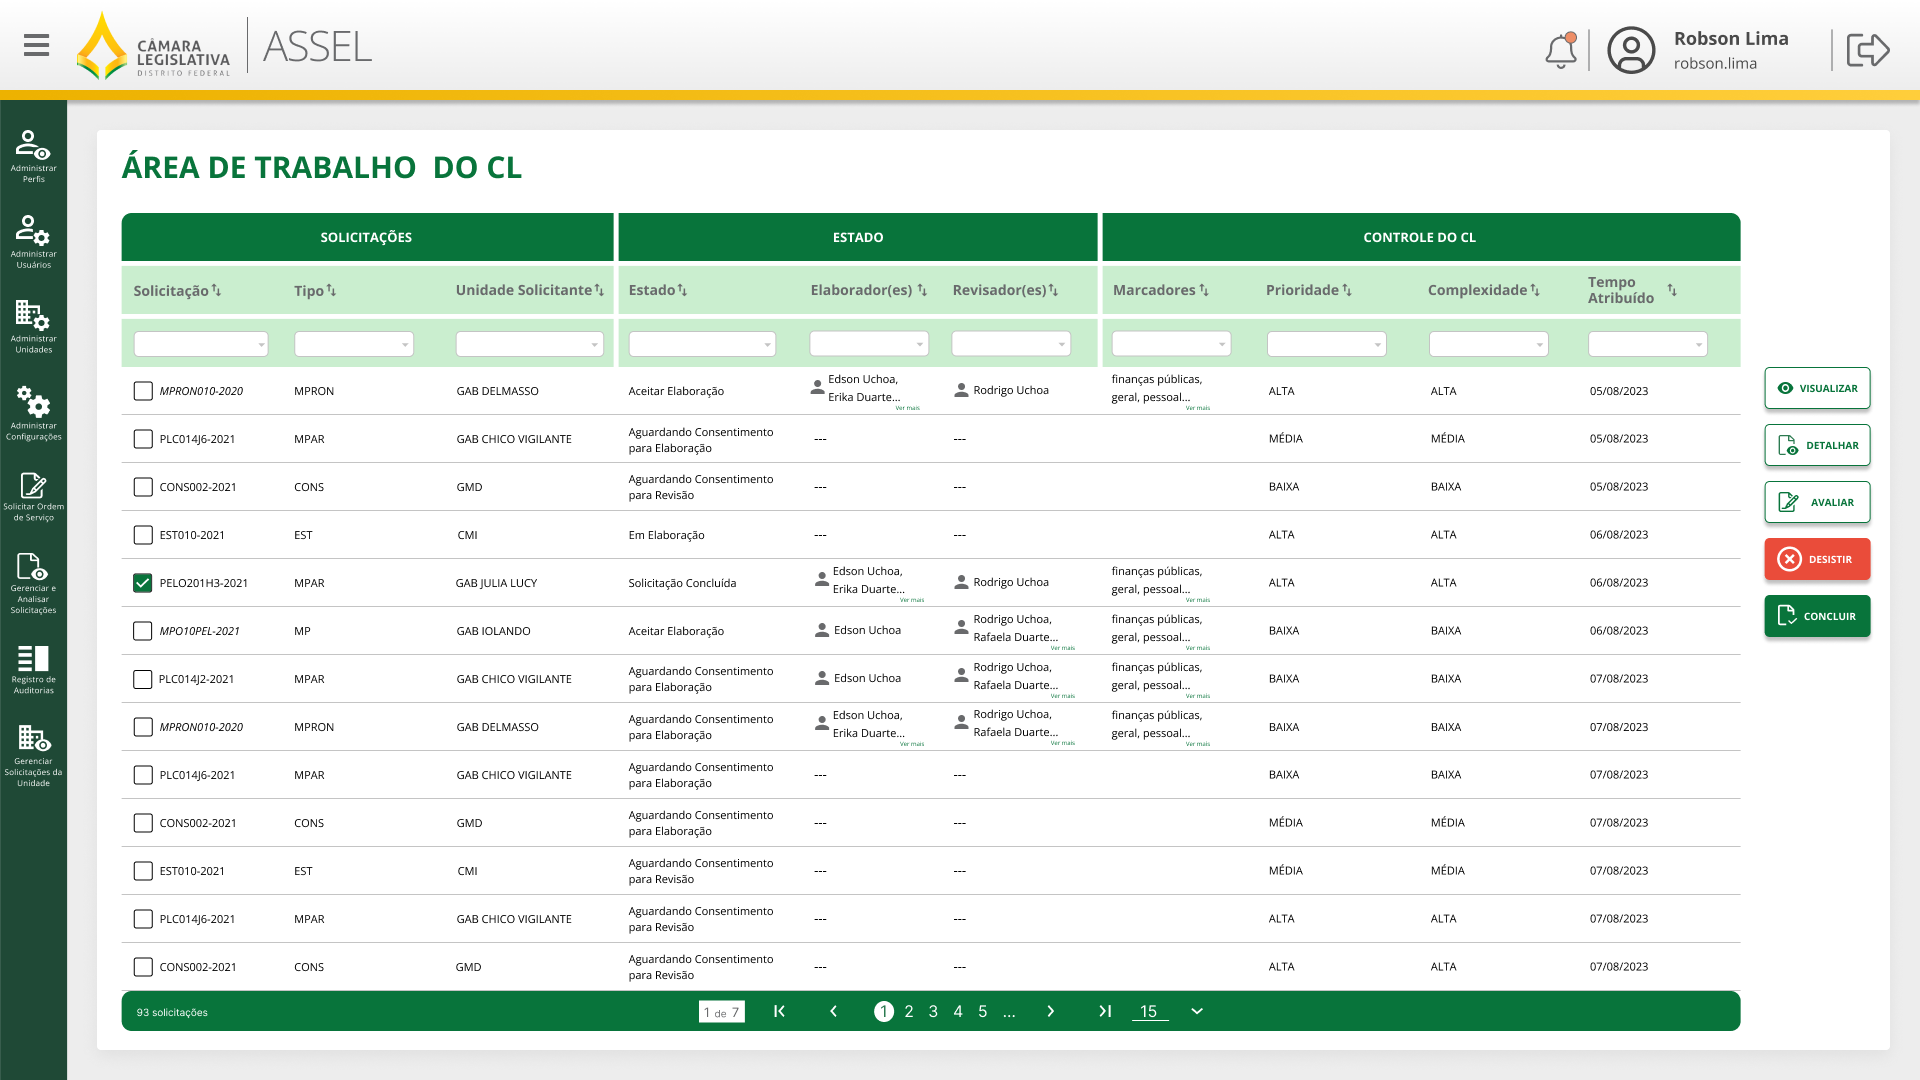
\includegraphics[width=0.99\linewidth]{AreaTrabalhoCL.png}
	\end{figure}
\end{frame}
% ------------------------------------------------------------
\begin{frame}
	\frametitle{Módulos das Unidades}
	\framesubtitle{Módulo Área de Trabalho do Consultor Legislativo - Objetivo}
	
	\begin{exampleblock}{Objetivos do Módulo ``Área de Trabalho do Consultor Legislativo''} 
		\begin{itemize}
			\item Gerenciamento pelo Consultor Legislativo da sua própria carga de trabalho na unidade;
			\item Gerenciamento de atividades de elaboração e revisão;
			\item Upload dos arquivos finais;
			\item Ferramentas:
			\begin{itemize}
				\item Relacionamentos entre solicitações;
				\item Acesso à consulta (a ser desenvolvida);
			\end{itemize}
			
		\end{itemize}
	\end{exampleblock}
\end{frame}
% =========================================================
\section{Módulo Minhas Notificações}

\begin{frame}
	\frametitle{Módulos das Unidades}
	\framesubtitle{Módulo Minhas Notificações}
	\begin{figure}
		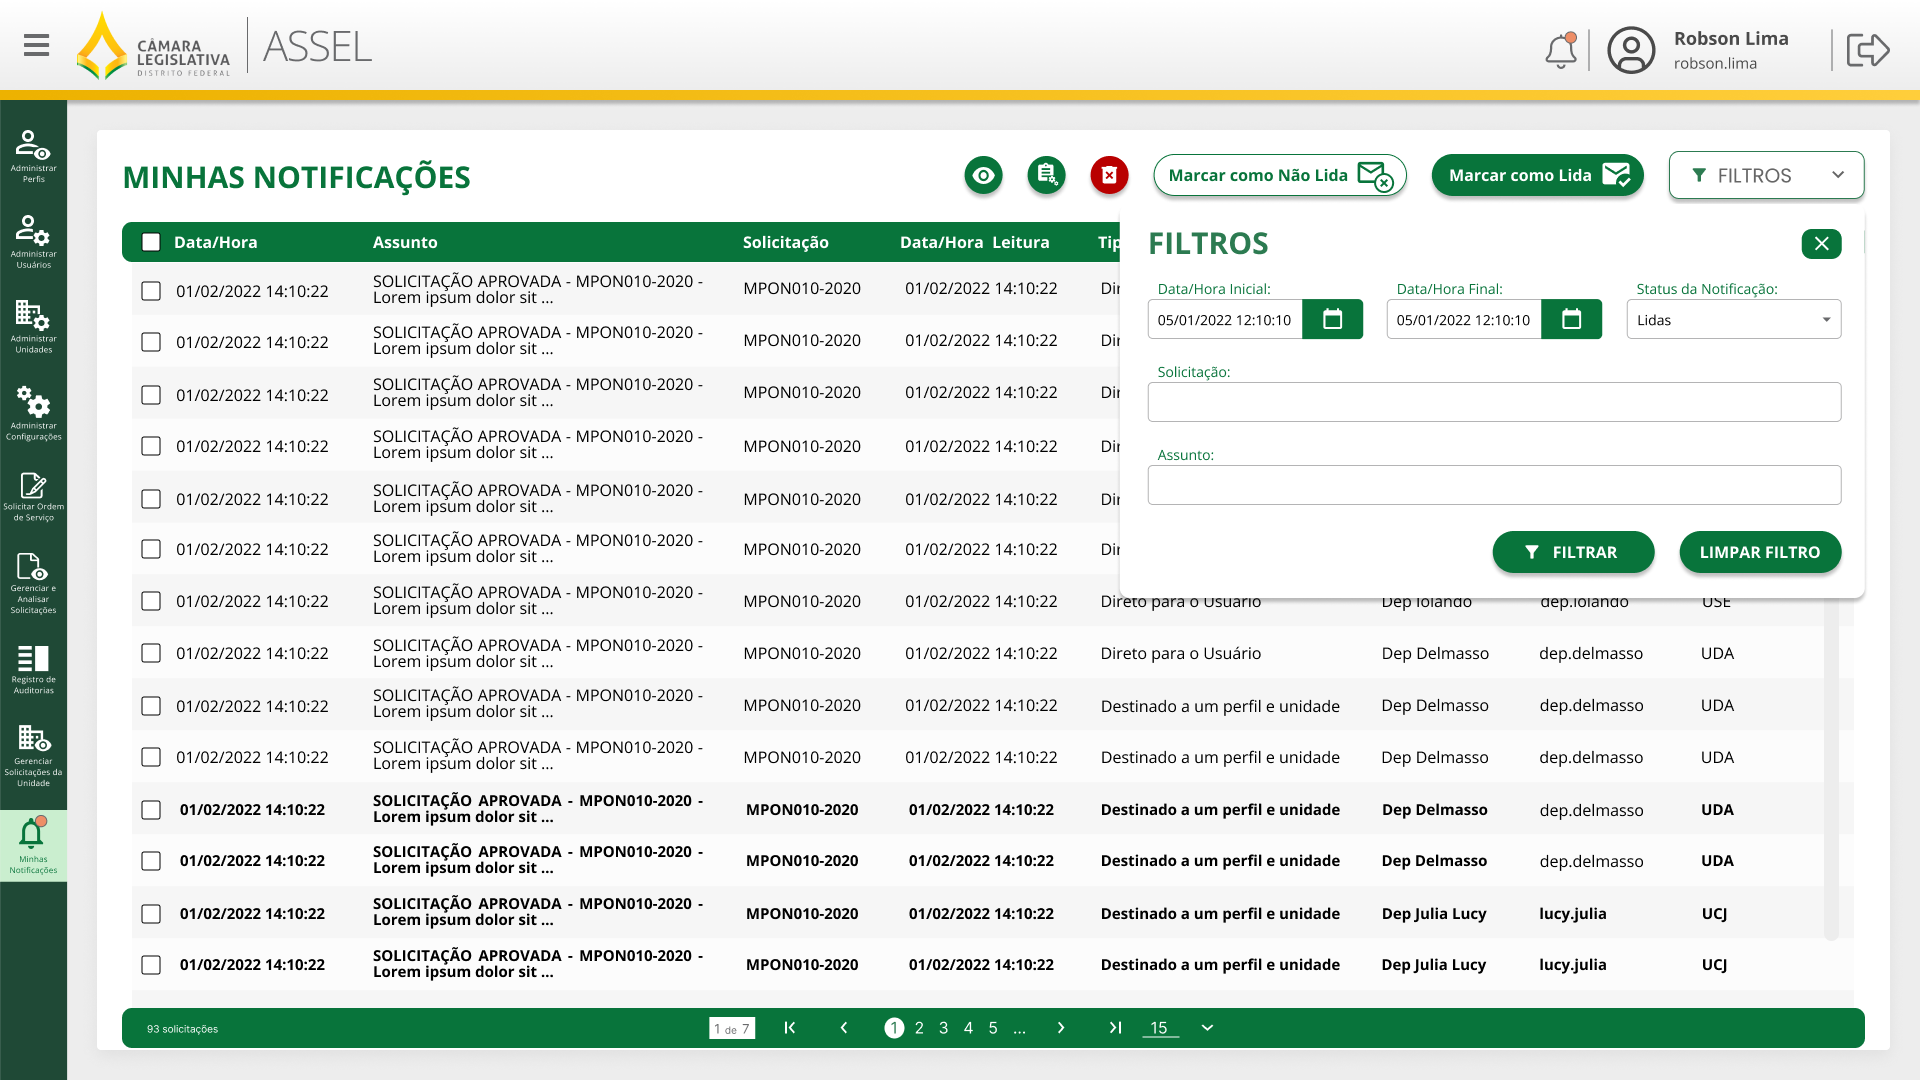
\includegraphics[width=0.99\linewidth]{MinhasNotificacoes.png}
	\end{figure}
\end{frame}
% ------------------------------------------------------------
\begin{frame}
	\frametitle{Módulos das Unidades}
	\framesubtitle{Módulo Minhas Notificações - Objetivo}
	
	\begin{exampleblock}{Objetivo} 
		\begin{itemize}
			\item Gerenciamento pelos usuários das notificações que receberam no sistema;
		\end{itemize}
	\end{exampleblock}
\end{frame}

% =========================================================

\section{Módulos das Unidades da Assessoria Legislativa}
\begin{frame}
	\frametitle{Módulos das Unidades}
	\framesubtitle{Observações}
	
	
	\begin{block}{Módulos das Unidades}
		\begin{itemize}
			\item Os três módulos funcionarão em conjunto;
			\item Permitir troca de informações entre os diversos atores de uma mesma Unidade de modo assíncrono:
			\begin{itemize}
				\item Teletrabalho;
			\end{itemize}
		\end{itemize}
	\end{block}	
\end{frame}
% =======================================


\section{Módulo Gerenciar Solicitações da Unidades - Funcionalidades}


\subsection{Visualizar, Detalhes e Classificação}

\begin{frame}
	\frametitle{Módulo Gerenciar Solicitações da Unidades}
	\framesubtitle{Funcionalidades}
	
	\textbf{Apresentação das Funcionalidades}
	
	\begin{alertblock}{Funcionalidades}
		\begin{enumerate}
			\item Funcionalidade ``Visualizar'';
			\item Funcionalidade ``Detalhes'';
			\item Funcionalidade ``Classificação'';
		\end{enumerate}
	\end{alertblock}	

	\begin{block}{} % Block without title
	\footnotesize Apresentar as funcionalidades usando a apresentação do protótipo. \normalsize
	\end{block}
	

\end{frame}



\begin{frame}
	\frametitle{Módulo Gerenciar Solicitações da Unidades}
	\framesubtitle{Estados Internos}

	\textbf{Estados Internos de uma Solicitação}

	\begin{figure}
		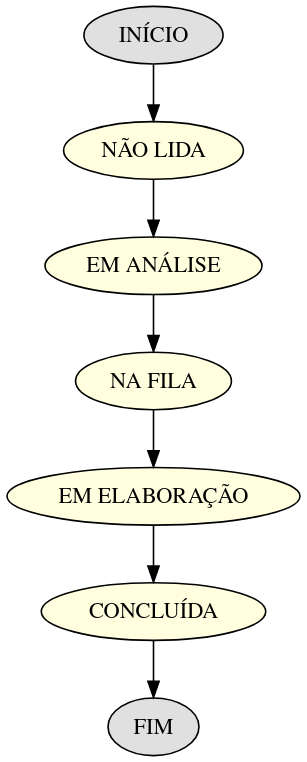
\includegraphics[width=0.2\linewidth]{fluxoBasico.png}
	\end{figure}
\end{frame}


\begin{frame}
	\frametitle{Módulo Gerenciar Solicitações da Unidades}
	\framesubtitle{Estados Internos}
	\begin{itemize}
		\item \textbf{Estado ``Não Lida''};
		\begin{itemize}
			\item Unidade ASSEL envia a solicitação para a Unidade fazendo-a aparecer na tabela de solicitações.
		\end{itemize}
	
		\item \textbf{Estado ``Em Análise''};
		\begin{itemize}
			\item Supervisor da Unidade seleciona a Solicitação e clica em ``Visualizar'' ou em ``Gerenciar Atribuições'' ou ainda em ``Analisar''.
		\end{itemize}
	
		\item \textbf{Estado: ``Na Fila''};
		\begin{itemize}
			\item Solicitações no estado ``Na Fila'' estão aguardando a alocação de Consultores;

			\item Se configurado, esse estado permite que os Consultores se inscrevam para atuarem como elaboradores.			
		\end{itemize}
	\end{itemize}
\end{frame}


\begin{frame}
	\frametitle{Módulo Gerenciar Solicitações da Unidades}
	\framesubtitle{Estados Internos - Em Elaboração}
	\begin{itemize}
		\item \textbf{Estado: ``Em Elaboração''};
		\begin{itemize}
			\item O estado ``Em Elaboração'' informa que uma dada solicitação está sendo desenvolvida por um ou mais Consultores. 
		\end{itemize}
	\end{itemize}

	\begin{block}{Elaboração e Revisão}
		\begin{itemize}
			\item A \textbf{Revisão} é uma atividade que acontece dentro do estado \textbf{``Em Elaboração''}.
			\item Isso permite manter a flexibilidades das diversas dinâmicas de elaboração e revisão dos trabalhos atualmente praticadas por cada unidade.
		\end{itemize}
	\end{block}
\end{frame}

\begin{frame}
	\frametitle{Módulo Gerenciar Solicitações da Unidades}
	\framesubtitle{Estados Internos - Estado Conclusão}
	\begin{itemize}
		\item \textbf{Estado: ``Conclusão''};
		\begin{itemize}
			\item Solicitações no estado ``Conclusão da Solicitação'' são elegíveis para serem encaminhados de volta para a ASSEL pelo Supervisor da Unidade. 
		\end{itemize}
	\end{itemize}
\end{frame}

\begin{frame}
	\frametitle{Módulo Gerenciar Solicitações da Unidades}
	\framesubtitle{Funcionalidades - Analisar}

	\textbf{Funcionalidade ``Analisar''}

	\begin{block}{Apresentação do Protótipo}
		\begin{itemize}
			\item Funcionalidade ``Analisar''
			\item Resultados:
			\begin{itemize}
				\item Aceitar e Colocar na Fila;
				\item Retorno (Devolução);
			\end{itemize}
		\end{itemize}
	\end{block}	
\end{frame}

\subsection{Distribuição Interna de Solicitações}

\begin{frame}
	\frametitle{Funcionalidades}
	\framesubtitle{Distribuição Interna de Solicitações}

	\textbf{Distribuição Interna de Solicitações}
	\begin{block}{Apresentação do Protótipo}
		\begin{itemize}
			\item ``Empurrar'' x  ``Puxar''
			\item Configurações
		\end{itemize}
	\end{block}	
\end{frame}


\begin{frame}
	\frametitle{Funcionalidades - Distribuição Interna de Solicitações}
	\framesubtitle{Empurrar x Puxar}

	\begin{itemize}
		\item \textbf{Empurrar = Atribuição pelo Supervisor}
		\item \textbf{Puxar = Inscrição pelo Consultor}
	\end{itemize}


		\begin{block}{Atribuição pelo Supervisor}
			\begin{itemize}
				\item Requer aceite ou rejeição pelo Consultor atribuído;
				\item Rejeição de atribuição pelo Consultor possui efeito imediato (não requer que o supervisor aceite ou recuse a rejeição);
			\end{itemize}
		\end{block}	


		\begin{block}{Inscrição pelo Consultor}
			\begin{itemize}
				\item Pode requerer Aprovação ou Recusa do Supervisor caso assim esteja configurado.
				
				\item Recusa de inscrição pelo Supervisor possui efeito imediato (não requer que o Consultor aceite ou rejeite a recusa);
			\end{itemize}
		\end{block}	



	\end{frame}



\subsection{Encaminhar}

\begin{frame}
	\frametitle{Funcionalidades}
	\framesubtitle{Encaminhar}
	
	\textbf{Encaminhamento de Solicitações Concluídas}
	
	\begin{block}{Apresentação do Protótipo}
		\begin{itemize}
			\item Encaminhar
		\end{itemize}
	\end{block}	

\end{frame}

\section{Próximos Passos}

\begin{frame}
	\frametitle{Próximos Passos}

	\begin{exampleblock}{Atualmente:}
		\begin{itemize}
			\item Módulo Gerenciar Solicitações das Unidades
			\item Módulo Área de Trabalho do CL
			\item Módulo de Minhas Notificações
		\end{itemize}
	\end{exampleblock}	

	\begin{block}{Para colocar em produção:}
		\begin{itemize}
			\item Módulo de Consulta
			\item Migração de Dados 
		\end{itemize}
	\end{block}	

	\begin{alertblock}{Futuro}
		\begin{itemize}
			\item Estatísticas e métricas de desempenho
			\item IA e BI
		\end{itemize}
	\end{alertblock}	
\end{frame}



\section{Feedback}

\begin{frame}
	\frametitle{Feedback}

	\begin{itemize}
		\item Feedback
	\end{itemize}
\end{frame}
